\uuid{zqC4}
\exo7id{745}
\auteur{bodin}
\organisation{exo7}
\datecreate{1998-09-01}
\isIndication{true}
\isCorrection{true}
\chapitre{Fonctions circulaires et hyperboliques inverses}
\sousChapitre{Fonctions circulaires inverses}

\contenu{
\texte{
Une statue de hauteur $s$ est placée sur un 
piédestal de hauteur $p$.
}
\begin{enumerate}
    \item \question{\`A quelle distance $x_0$ doit se placer un observateur
(dont la taille est supposée négligeable) pour voir la statue sous un 
angle maximal $\alpha_0$?}
\reponse{On note $x$ la distance de l'observateur au pied de la statue.
On note $\alpha$ l'angle d'observation de la statue seule, et $\beta$
l'angle d'observation du piédestal seul.

\begin{center}
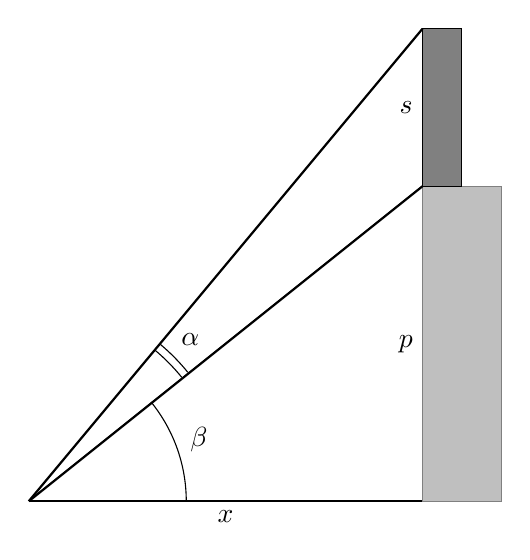
\begin{tikzpicture}[scale=1]

\filldraw[fill=gray!50, draw=gray] (5,0)--(6,0)--(6,4)--(5,4)--cycle;
\filldraw[fill=gray, draw=black] (5,4)--(5.5,4)--(5.5,6)--(5,6)--cycle;
\draw[thick] (0,0)--(5,0);
\draw[thick] (0,0)--(5,4);
\draw[thick] (0,0)--(5,6);
 
 \node at (5,5) [left] {$s$};    
 \node at (5,2) [left] {$p$};  
 \node at (2.5,0) [below] {$x$};  

\draw (2,0) arc(0:39:2) ;
\draw (39:2.5) arc(39:50:2.5) ;
\draw (39:2.6) arc(39:50:2.6) ;

\node at (45:2.9)  {$\alpha$};  
\node at (20:2.3)  {$\beta$};  
\end{tikzpicture}
\end{center}

Nous avons les relations trigonométriques dans les triangles rectangles :
$$\tan(\alpha+\beta) = \frac{p+s}{x} \qquad\text{ et }\qquad \tan\beta = \frac{p}{x}$$
On en déduit les deux identités :
$$\alpha+\beta = \Arctan\left(\frac{p+s}{x}\right) \qquad\text{ et }\qquad \beta = \Arctan\left(\frac{p}{x}\right)$$
à partir desquelles on obtient $\alpha=\alpha(x)=\Arctan\left(\frac{p+s}{x}\right)-\Arctan\left(\frac{p}{x}\right)$.

\'Etudions cette fonction sur $]0,+\infty[$ : elle est dérivable et 
$$\alpha'(x)=\frac{-\frac{s+p}{x^2}}{1+\left(\frac{s+p}{x}\right)^2}-\frac{-\frac{p}{x^2}}{1+\left(\frac{p}{x}\right)^2}=\frac{s}{(x^2+p^2)(x^2+(s+p)^2)}\big(p(p+s)-x^2\big)$$
Ainsi $\alpha'$ ne s'annule sur $]0,+\infty[$ qu'en $x_0 = \sqrt{p(p+s)}$.
Par des considérations physiques, à la limite en $0$ et en $+\infty$, 
l'angle $\alpha$ est nul,
alors en $x_0$ nous obtenons un angle $\alpha$ maximum.
Donc la distance optimale de vision est  $x_0 = \sqrt{p(p+s)}$.}
    \item \question{Vérifier que $\alpha_0=\Arctan \frac{s}{2\sqrt{p(p+s)}}$.}
\reponse{Pour calculer l'angle maximum $\alpha_0$ correspondant, on pourrait 
calculer $\alpha_0 = \alpha(x_0)$ à partir de la définition de la fonction
$\alpha(x)$. Pour obtenir une formule plus simple nous 
utilisons la formule trigonométrique suivante : si
$a$, $b$ et $a-b$ sont dans l'intervalle de définition de la fonction $\tan$, alors
$\tan(a-b)=\frac{\tan a-\tan b}{1+\tan a \tan b}$, ce qui donne ici
$$\tan\alpha_0 = \tan\big( (\alpha_0+\beta_0) - \beta_0 \big)
=\frac{\frac{p+s}{x_0}-\frac{p}{x_0}}{1+\frac{p+s}{x_0}\cdot\frac{p}{x_0}}
= \frac{s}{2x_0}=\frac{s}{2\sqrt{p(p+s)}}$$
Comme $\alpha_0\in]-\frac{\pi}{2},\frac{\pi}{2}[$, 
on en déduit $\alpha_0 = \Arctan \frac{s}{2x_0} = \Arctan \frac{s}{2\sqrt{p(p+s)}}$.}
    \item \question{Application à la statue de la liberté : haute de $46$ mètres avec un piédestal de 
$47$ mètres.}
\reponse{Pour la statue de la liberté, on a la hauteur de la statue $s=46$ mètres
et la hauteur du piédestal $p=47$ mètres.
On trouve donc 
$$x_0 = \sqrt{p(p+s)} \simeq 65,40 \text{mètres} \qquad 
\alpha_0 = \Arctan \frac{s}{2\sqrt{p(p+s)}} \simeq 19^\circ.$$

Voici les représentations de la statue et de la fonction $\alpha(x)$ pour ces valeurs de $s$
et $p$.}
\indication{Faire un dessin. Calculer l'angle d'observation $\alpha$ en fonction de la distance $x$
et étudier cette fonction. Pour simplifier l'expression de $\alpha_0$, 
calculer $\tan\alpha_0$ à l'aide de la formule donnant $\tan(a-b)$.}
\end{enumerate}
}
